%! Author = itgramic
%! Date = 26.01.24

% Preamble
%\subsubsection{Monolitische Umgebung}
%\subsubsection{Kubernetes}
%\begin{flushleft}
%    Um ein minimales, dem Produktiven möglichst nahes Enviroment für die evaluation zu erhalten, wurde folgendes Setting ausgewählt:
%    \begin{figure}[H]
%        \centering
%        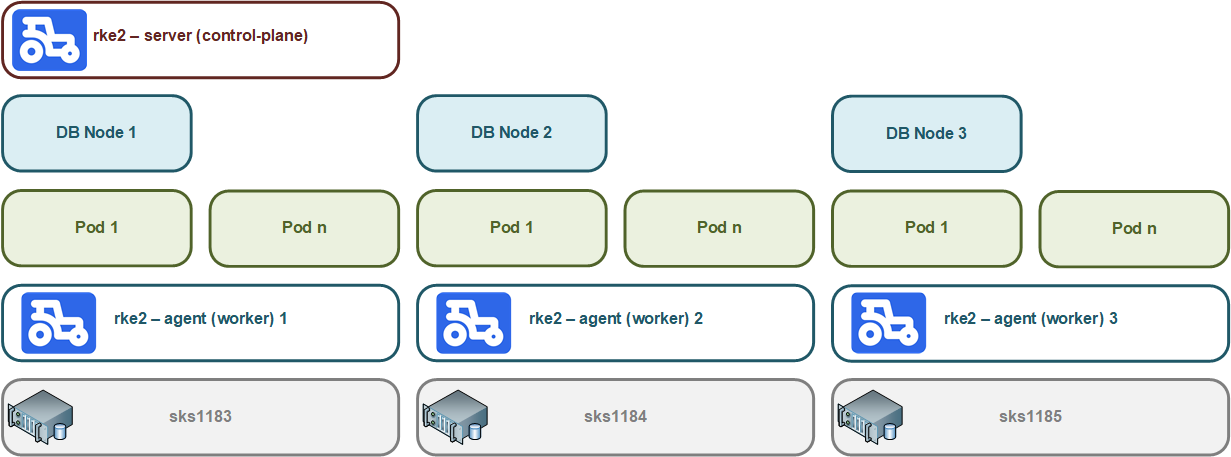
\includegraphics[width=1\linewidth]{source/implementation/evaluation/platforms/evaluation_enviroment_rke2}
%        \caption{Kubernetes - Evaluations-Enviroment}
%        \label{fig:k8s_evalution_enviroment}
%    \end{figure}
%\end{flushleft}
%\begin{flushleft}
%    Die genauen Spezifikationen sind wie folgt:
%    \begin{table}[H]
%    \begin{tabular}{ll}
%    \textbf{Linux Distribution}                & Debian 11              \\
%    \textbf{Kubernetes Runtime}                & rke2                   \\
%    \textbf{Container-Enviroment}              & containerd             \\
%    \textbf{Container Network Interface (CNI)} & cilium                 \\
%    \textbf{Cloud Native Storage (CNS)}        & local-path-provisioner
%    \end{tabular}
%    \caption{Evaluations settings}
%    \label{tab:evaluation-setting}
%    \end{table}
%\end{flushleft}

\begin{flushleft}
    Entsprechend wurden folgende Server bereitgestellt:
    \begin{longtable}[H]{lllll}

\toprule
Server & Typ & Funktion & Full Qualified Device Name & IP \\
\midrule
\endfirsthead
\caption[]{Evaluationssyssteme} \\
\toprule
Server & Typ & Funktion & Full Qualified Device Name & IP \\
\midrule
\endhead
\midrule
\multicolumn{5}{r}{Continued on next page} \\
\midrule
\endfoot
\bottomrule
\endlastfoot
sks1183 & Distributed SQL & Server & sks1183.ksgr.ch & 10.0.20.97 \\
sks1184 & Distributed SQL & Agent & sks1184.ksgr.ch & 10.0.20.104 \\
sks1185 & Distributed SQL & Agent & sks1185.ksgr.ch &  10.0.20.105 \\
vks0032 & Distributed SQL & Virteulle IP & vks0032.ksgr.ch & 10.0.20.106 \\
\caption{Evaluationssyssteme} \label{evaluation_inventory}
\end{longtable}

\end{flushleft}